% File emnlp2018.tex
%
%% Based on the style files for EMNLP 2018, which were
%% Based on the style files for ACL 2018, which were
%% Based on the style files for ACL-2015, with some improvements
%%  taken from the NAACL-2016 style
%% Based on the style files for ACL-2014, which were, in turn,
%% based on ACL-2013, ACL-2012, ACL-2011, ACL-2010, ACL-IJCNLP-2009,
%% EACL-2009, IJCNLP-2008...
%% Based on the style files for EACL 2006 by 
%%e.agirre@ehu.es or Sergi.Balari@uab.es
%% and that of ACL 08 by Joakim Nivre and Noah Smith

\documentclass[11pt,a4paper]{article}
\usepackage[hyperref]{emnlp2018}
\usepackage{times}
\usepackage{latexsym}

\usepackage{url}
\special{papersize=210mm,297mm}

\aclfinalcopy % Uncomment this line for the final submission

%\setlength\titlebox{5cm}
% You can expand the titlebox if you need extra space
% to show all the authors. Please do not make the titlebox
% smaller than 5cm (the original size); we will check this
% in the camera-ready version and ask you to change it back.

\newcommand\BibTeX{B{\sc ib}\TeX}
\newcommand\confname{EMNLP 2018}
\newcommand\conforg{SIGDAT}

\title{Controlling Length in Abstractive Summarization Using a Convolutional
Neural Network}


\date{}

\usepackage{url}

\usepackage{times}
\usepackage{helvet}
\usepackage{courier}
\usepackage{color}
\usepackage{amsmath,amsfonts,amssymb,amsthm,amsopn}
\usepackage{times}
\usepackage{url}
\usepackage{color}
\usepackage{latexsym}
\usepackage{epsfig}
\usepackage{graphicx}
\usepackage{booktabs}
%\usepackage{diagbox}
\usepackage{array}
\usepackage{multicol}
\usepackage{threeparttable}
\usepackage{epstopdf}
\usepackage{listings}
\usepackage{multirow}
\usepackage{subfigure}
%\usepackage{subfig}

%\aclfinalcopy % Uncomment this line for the final submission
%\def\aclpaperid{***} %  Enter the acl Paper ID here

%\setlength\titlebox{5cm}
% You can expand the titlebox if you need extra space
% to show all the authors. Please do not make the titlebox
% smaller than 5cm (the original size); we will check this
% in the camera-ready version and ask you to change it back.
%\newcommand\BibTeX{B{\sc ib}\TeX}
%code environment
%\definecolor{dkgreen}{rgb}{0,0.6,0}
%\definecolor{gray}{rgb}{0.5,0.5,0.5}
%\definecolor{mauve}{rgb}{0.58,0,0.82}
%\lstset{frame=tb,
%  language=Java,
%  aboveskip=1.5mm,
%  belowskip=1.5mm,
%  showstringspaces=false,
%  columns=flexible,
%  basicstyle={\tiny\ttfamily},
%  numbers=none,
%  keywordstyle=\tiny\color{blue},
%  numberstyle=\tiny\color{gray},
%  commentstyle=\tiny\color{dkgreen},
%  stringstyle=\tiny\color{mauve},
%  breaklines=true,
%  breakatwhitespace=true
%  tabsize=3
%}

\newcommand{\secref}[1]{Section \ref{#1}}
\newcommand{\figref}[1]{Figure \ref{#1}}
\newcommand{\eqnref}[1]{Eq. (\ref{#1})}
\newcommand{\tabref}[1]{Table \ref{#1}}
\newcommand{\exref}[1]{Example \ref{#1}}
\newcommand{\cut}[1]{}
\newcommand{\tabincell}[2]{\begin{tabular}{@{}#1@{}}#2\end{tabular}}

\newcommand{\KZ}[1]{\textcolor{blue}{Kenny: #1}}
\newcommand{\YZ}[1]{\textcolor{red}{Yizhu: #1}}
\newcommand{\ZY}[1]{\textcolor{green}{Zhiyi: #1}}

\begin{document}


\author{
 Yizhu Liu$^1$ \hspace*{1cm}
 Zhiyi Luo$^2$  \hspace*{1cm}
 Kenny Q. Zhu$^3$ 
 \\ 
 Shanghai Jiao Tong University, Shanghai, China \\
 \{$^1$liuyizhu, $^2$jessherlock\}@sjtu.edu.cn,
 $^3$kzhu@cs.sjtu.edu.cn
 }

\maketitle

\begin{abstract}
Convolutional neural networks (CNNs) have met great success
in abstractive summarization, but they
cannot effectively generate summaries
of desired lengths. Because generated summaries are used in difference
scenarios which may have space or length constraints,
the ability to control the summary length in abstractive summarization
is an important problem. In this paper, we propose an approach
to constrain the summary length by extending a convolutional
sequence to sequence model.  The results show that this approach 
generates high-quality summaries with user defined length, 
and outperforms the baselines consistently in terms of
ROUGE score, length variations and semantic similarity.
%Our model can generate summraies in any length as well as any length range.
%We consistently achieve higher ROUGE score than previous methods under
%various length constraints.
\end{abstract}

\section{Introduction}

Protein$-$protein interactions (PPIs) are of central importance for the majority of biological functions, such as signal transduction, metabolic pathways, molecular dynamics, and protein networks\cite{Hoffmann.Krallinger.ea:2005}, for they serve as the most fundamental building blocks of the entire interacademic systems of any organisms. Collecting data on pairwise interaction relationships is essential for multiple purpose, including identification of modules with certain functionality\cite{Spirin.Mirny.03}, mapping diseases to dominated genes\cite{Ideker.Sharan.08}, and after all, understanding wholistic metabolic/genetic networks from a system biology perspective.

A lot of databases have been built to store protein and genetic interactions from major model organism species and are available in various standardized formats, such as MINT\cite{Zanzoni.Montecchi-Palazzi.ea:2002}, BIND\cite{Bader.ea:2003}, BIOGRID\cite{DBLP:journals/nar/StarkBRBBT06}, etc. Among those mainstream databases, the data largely rely on voluntary reports by scientists or researchers, besides, comprehensive curation efforts become indispensable for the sake of accuracy. However, the amount of biology-related literatures with respect to protein interactions grows explosively and thus make it either impossible or impractical to manually detect PPI information anymore.

Considering huge amount of PPI information with great wealth hidden in published papers, in recent years, numerous mining techniques have been proposed that aim to extract PPI information automatically from free text, especially machine learning, information retrieval, and natural language processing\cite{DBLP:journals/bib/WinnenburgWPDS08}.These approaches can be roughly categorized into three classes: co$-$occurrence, rule$-$based, and machine learning. 

Co$-$occurrence is the approach with most simplicity and naivete. Just as its name implies, this method intends to find out pairs of proteins that co-occur in the same context. The scope of "same context" ranges from phrase, sentence, paragraph to whole abstract, even document. The underlying assumption is that whenever two proteins are mentioned together by authors, chances are high that there is some kind of relationship between them. However, however, in-context closeness even semantic relation does not necessarily represent actual biological interaction. As a consequence, a large fraction of candidate pairs are mismatched inevitably, causing a high recall but low precision.

The second approach is rule-based extraction, in other words, pattern matching. There are many types of rules, most of them concern natural language processing (NLP). One way is to specify hand-crafted regular expressions before hand, which mostly lean on language usage preference. Besides, by using full or partial (shallow) parsing strategies, more information would be acquired, such as part-of-speech taggers, local dependencies between syntactic components, context-free grammar\cite{DBLP:journals/bioinformatics/TemkinG03}, and full sentence structure. Compared to co$-$occurrence, rule-based approach enjoy better precision but much lower recall. In addition, since the rules are usually derived from training data, that is to say, the improper choice of training data would be significantly lethal, therefore quality of extraction is invariably instable and may not applicable to other data.

The third and most commonly used approach use machine learning techniques, in this case, the task to extract protein$-$protein interactions turns out to be a binary classification problem. Each protein pairs are represented along with a set of features, which is associated with their context, then a well$-$defined classifier gives the answer whether the candidate protein pairs is classified to be qualified PPI. (TO BE FURTHER FILLED!!!)

In this paper, we introduce a general bootstrapping framework for Protein$-$protein interaction extraction from natural text.Our method differs from most of the previous works in three aspects:

(1)The extraction process is driven by only tiny fraction of training data, which are regarded as seed data. In each round, it would derive reliable patterns automatically from seed data, then extract more positive PPI pairs consequently, what's more, the seed data would be augmented by the newly extracted results with high confidence.

(2)multiple graph kernel. 

(3)various evaluation.




%\section{Sentiment-Aspect-Region Model}
\label{sec:model}
We first present our objectives to build the
unified sentiment-aspect-region model.
To achieve the objectives, we present several intuitions
based on which we build our model.
We then describe the details of the model,
and propose a parameter estimation method.

\subsection{Intuitions}
\label{sec:motiv}
%We first introduce some notions that are used in
%explaining our objectives. There are three types of
%latent factors that are not observable in a geotagged review corpus, but
%are important for user preference analysis. They
%are topical-region, topical-aspect and sentiment.
%A topical-region represents a geographical area in which
%users do similar things (such as dining).
%%write region-specific words on their reviews.
%It comprises two components: geo-location and semantics.
%The geo-location component is usually modeled as a
%Gaussian distribution over
%POIs \cite{Yin:2011,YuanW4:2013}.
%The semantic component is modeled as a multinomial
%distribution over words \cite{Geofolk:2010}.
%Example topical-regions include shopping areas, education areas,
%streets of special snacks, etc.
%Topical-aspects are the aspects of POIs that
%are commented by users, such as environment, taste,
%price, etc. Sentiments are user's opinions over
%topical-aspects (e.g., positive, negative or neutral).
%%\KZ{Can sentiments be casted over regions? e.g., I hate
%%Clarke Quay!}
%Topical-aspects
%and sentiments can be modeled jointly \cite{JoASUM:2011}.

In this paper,
we aim at building a model that is able to 1) extract
latent variables, i.e., topical-aspect, sentiment,
and topical-region from the review
data; 2) capture the interdependencies among
category, POI, user, words and the three latent
variables; and 3) discover user's topical-region and
topical-aspect preferences.
To achieve these objectives,
we exploit the following intuitions in designing our model:

\textbf{Intuition 1}: A user visits POIs in a topical-region
because the region is geographically convenient to the user
(e.g., close to her activity areas) and its topics (e.g., shopping
street, education area, etc.) satisfy
the user's interest. Each user has her own preferences on the
topical-regions.
%We use a topical-region
%variable $r$ to model the mixture of topic and geographic
%information,
%i.e., each region exactly covers POIs of similar
%topic distribution and close in spatial.

\textbf{Intuition 2}: A user rates highly of a POI because
she likes some aspects of the POI. Such preferences might be
indicated in her review.
%i.e., user has preferences on some aspects of the POI.
Some users like to check the price range of a restaurant first while
others might be more concerned with the environment. Moreover, POIs in different
categories may have different aspects of interest.
%For
%instance, a traveler might care more about the environment
%of a hotel, while a hungry would-be diner might be more interested in
%the waiting time of a restaurant.

\textbf{Intuition 3}:
A user decides to visit a POI in a region
by considering the category, category-aware topical-aspects of the POI and
the distance to it. For example, users may visit POIs of the
restaurant category with good environment,
but she may first consider the restaurants nearby.
%to walk around a nearby shopping street.
%and visit
%POIs without being particular about the category.

\textbf{Intuition 4}: When a user writes a review on a POI, she
will use words for both the aspects of the POI and
her sentiments about the aspects.
The user may also use words for the topical-region of the POI.
For example, a review on a shop in Times Square may say:
``This shop offers best prices in Times Square.'' The reviewer
uses ``price'' for {\em aspect}, ``best'' for {\em sentiment}
and ``Times Square'' for {\em region}. %to construct the review.
%Moreover, each sentence in the review normally
%corresponds to exactly one aspect and
%users only associate one sentiment on each aspect. As a result,
%the words co-occurs in the same sentences are more likely to be correlated to
%the same aspect and sentiment.

\subsection{Model Description}
We first define the notations
to be used in the proposed model. Let $D$ be the set of user reviews,
and $U$ be the set of users. For each review, we denote the
number of its sentences by $M$ and number of words in each
sentence by $N$. In our model, a location has two attributes:
identifier and coordinates. We use $l$ to represent a location identifier
and $\boldsymbol{cd}_l$ to denote its corresponding coordinates.
Here $\boldsymbol{cd}_l$ is a latitude and longitude pair. We denote
the topical-aspect, sentiment and topical-region by $a$, $s$,
and $r$, respectively. The notations
used in this paper are listed in \tabref{tab:notation}.
Following the intuitions discussed in \secref{sec:motiv}, we
proceed to present our model.

\begin{table}[th]
\centering
%\scriptsize
\caption{Description of Symbols}
\begin{tabular}{l|l}
\hline
 Symbol & Description\\
\hline
$u$, $U$ & individual user and the set of users\\
\hline
$l$, $L$ & individual POI and the set of POIs  \\
\hline
$c$ & category  \\
\hline
$r$ & topical-region  \\
\hline
$a$, $s$ & topical-aspect and sentiment \\
\hline
$d$, $D$ & single review and the set of reviews \\
\hline
$M$ & the number of sentences in a review \\
\hline
$w$, $N$ & single word and the number of words in a sentence \\
\hline
\end{tabular}
\label{tab:notation}
\end{table}

Based on \textbf{Intuitions 1\&2}, we model the user
topical-region preferences and topical-aspect preferences
as multinomial distributions $p(r|u)$ and $p(a|u,c)$, respectively.

Based on \textbf{Intuition 3}, a user chooses a POI to visit
by considering both the category and the distance. We
define the probability of visiting a POI $l$ given
category $c$ and region $r$ proportional to $p(l|c)\cdot p(l|r)$.
Here $p(l|c)$ is the probability of selecting POI $l$ from
the category $c$; $p(l|r)$ is a the probability
of selecting POI $l$ in region $r$ by considering
the distance from $l$ to $r$. After normalization, we have the
definition $p(l|c,r)=\frac{p(l|c)p(l|r)}{\sum_{l'}{p(l'|c)p(l'|r)}}$.
%The denominator is used to normalize
%the $p(l|c)p(l|r)$ over all POIs.
To model the spatial distance, we use a
Gaussian mixture model, i.e.,
$p(l|r)\sim N(\boldsymbol{\mu}_r, \boldsymbol{\Sigma}_r)$, where
$\boldsymbol{\mu}_r$ is the center of region $r$ and
$\boldsymbol{\Sigma}_r$ is the co-variance matrix which depicts the
area of region $r$.
To model the membership of a POI to a category, we use a uniform
distribution for $p(l|c)$.
%$\kappa$ is tunable parameter used
%for balance the weights of generating POI from category and region.
%Note that $p(l|r)$ is a continuous distribution while $p(l|c)$ is
%a discrete distribution.
%To multiply the two distributions,
%we adopt the coordinate transformation approach for the Gaussian
%distribution that is proposed in Yuan et al.\cite{YuanW4:2013}.

Based on \textbf{Intuition 4},
we model the relationships among words, topical-aspects,
sentiments and topical-regions by
$p(w|a,s,r)=\lambda p(w|a,s)+(1-\lambda) p(w|r)$, where
$a$, $s$, $r$ are topical-aspect, sentiment and
topical-region, respectively.
Here $p(w|a,s)$ is the probability that the users write
word $w$ when they have sentiment $s$ on aspect $a$;
$p(w|r)$ is the probability that the users use word
$w$ to describe region $r$; parameter
$\lambda$ is used to balance the portion of
words drawn from topical-aspect, sentiment or topical-region.
We model $p(w|a,s)$ instead of $p(w|a)$ and $p(w|s)$
because aspects and sentiments are closely coupled,
and modeling by $p(w|a)$ and $p(w|s)$
needs an additional tuning parameter.
Similar to proposals of sentence level sentiment analysis
\cite{TitovMGLDA:2008,TitovMAS:2008, JoASUM:2011},
we assume each sentence expresses opinions on exactly one topical-aspect
and each topical-aspect is associated to a positive, negative or neutral sentiment.

\begin{figure}[th]
\centering
\epsfig{file=fig/modeldraft.eps,width=0.65\columnwidth}
\caption{Sentiment-Aspect-Region Model (SAR)}
\label{fig:model}
\end{figure}

In summary, the graphical representation of our model
is shown in \figref{fig:model} and
the generative process of the
reviews written by user $u$ is described as follows:
\begin{itemize}
\item For each review $d\in D_u$, where $D_u$ is the set of reviews written by user $u$.
    \begin{itemize}
    \item Draw topical region $r\sim p(r|u)$
    \item Draw category $c\sim p(c|u)$
    \item Draw location $l\sim p(l|c,r)=\frac{p(l|r)p(l|c)}{\sum_{l'}{p(l'|c)p(l'|r)}}$, where $p(l|r)\sim N(\boldsymbol{\mu}_r,\boldsymbol{\Sigma}_r)$
    \item For each sentence in review $d$
        \begin{itemize}
        \item Draw aspect $a\sim p(a|u,c)$
        \item Draw sentiment $s\sim p(s|a,l)$
        \item For each word position in the sentence
            \begin{itemize}
            \item Draw word $w\sim p(w|a,s,r)={\lambda}p(w|a,s)+(1-\lambda)p(w|r)$
            \end{itemize}
        \end{itemize}
    \end{itemize}
\end{itemize}

In the model, $p(l|c)$ and
$p(c|u)$ can be estimated directly from a given corpus. The
other distribution parameters need to be inferred.
We first present how to estimate $p(l|c)$ and
$p(c|u)$, and then show the inference algorithm for
the remaining distributions in \secref{sec:infer}.

As described in \textbf{Intuition 3},
a POI $l$ is generated from both category
and region. Since POI $l$ and category $c$ are
observable variables, we simply compute $p(l|c)$
by \equref{eq:plc}.
\begin{equation}
p(l|c)=\frac{I(l,c)}{\#\; of\; POIs\; in\; c}
\label{eq:plc}
\end{equation}
\begin{equation}
I(l,c)=
\begin{cases}
1 & l\in c \\
0 & otherwise \\
\end{cases}
\end{equation}

Similarly, we compute the category preferences of each user, i.e., $p(c|u)$,
directly from the corpus. To handle the overfitting problem,
we apply the additive smoothing technique. After smoothing, even though a user did
not a visit some category of POIs, the probability of
visiting that category still has a small value. The computation of $p(c|u)$ is shown in
\equref{eq:pcu}.
\begin{equation}
p(c|u)=\frac{n_c+\alpha}{N+{\alpha}C},
\label{eq:pcu}
\end{equation}
where $n_c$ is the number of reviews of POIs in category $c$ that user $u$
writes; $N$ is the total number of reviews on POIs in $c$; $C$
is the total number of categories; $\alpha$  is the smoothing
parameter which is usually set to a value smaller than 1. In this paper,
we set $\alpha=0.1$.

\subsection{Inference Algorithm}
\label{sec:infer}
To infer the parameters of the model, we
use the expectation-maximization (EM) approach.
In this section,
we present the computation of the corpus
likelihood, the two-step EM algorithm
used to infer our parameters, and
initialization of the EM algorithm.

\subsubsection{Likelihood Computation}
Our model has several levels, i.e., word level,
sentence level, and document level. The latent variables
are on two levels. Region $r$ is at document level while
aspect $a$ and sentiment $s$ are at sentence level.
This multi-level structure poses challenges to the estimation of
the log-likelihood. According to the generative
process, we have the likelihood of the corpus $D$:
\begin{equation}
p(D;\Phi)=\prod_{d}^{D}{p(u_d)\sum_{r}^{R}{p(r|u_d)}p(l_d,\mathbf{w}_d|r,u_d)}
\label{eq:likeli1}
\end{equation}
\begin{equation}
p(l_d,\mathbf{w}_d|r,u_d)=p(c_{l_d}|u_d)p(l_d|r,c_{l_d})\prod_{i}^{M}{p(\mathbf{w}_{d,i}|c_{l_d},r,u_d,l_d)}
\label{eq:likeli2}
\end{equation}
\begin{equation}
\begin{split}
&p(\mathbf{w}_{d,i}|c_{l_d},r,u_d,l_d) \\
&=\sum_{a,s}{p(a|c_{l_d},u_d)p(s|a,l_d)\prod_{j}^{N}{p(w_{d,i,j}|a,s,r)}}
\end{split}
\label{eq:likeli3}
\end{equation}
In \equref{eq:likeli1}, $\Phi$ is the set of parameters in the model,
i.e., $p(r|u)$, $p(a|c,u)$,$p(l|r)$,$p(s|a,l)$,$p(w|a,s)$,
$p(w|r)$,$\boldsymbol{\mu}_r$ and $\boldsymbol{\Sigma}_r$.
Variables $u_d$,$l_d$,$\mathbf{w}_d$ are the user, location and
words of review $d$, respectively. Variable $\mathbf{w}_{d,i}$
represents the set of words in sentence $i$ of review $d$
while $w_{d,i,j}$ is the $j^{th}$ word in sentence
$i$ of review $d$. Taking logarithm of
$p(D;\Phi)$ leads to a summation inside the logarithm:
\begin{equation}
L=\sum_{d}{\log{p(u_d)}+\log{\sum_{r}{p(r|u_d)p(l_d,\mathbf{w}_d|r,u_d)}}}
\label{eq:loglikeli}
\end{equation}
Since this likelihood cannot be estimated directly,
we adopt Jessen's
inequality to the log-likelihood, and estimate the
lower bound of the likelihood and the parameters
in an iterative manner.

\subsubsection{Expectation-Maximization}
Due to the aforementioned difficulty of computing
log-likelihood directly,
we apply Expectation-Maximization (EM)
algorithm to estimate the model parameters.

In \textbf{E-step}, we compute the expectation
of latent variables given the observed data.
By applying Jessen's inequality to \equref{eq:loglikeli},
we get the lower bound of the likelihood as:
\begin{equation}
\begin{split}
L_{LB}=&\sum_{d}{\log{p(u_d)}}\\
+&\sum_{d,r}{p(r|d)(\log{p(r|u_d)}+\log{p(l_d,\mathbf{w}_d|r,u_d)})}
\end{split}
\label{eq:loglikeli1}
\end{equation}
As shown in \equref{eq:loglikeli1},
we need to estimate $p(r|d)$ to compute the full likelihood.
We apply Bayes rule, and obtain the update
function of the posterior distribution as
\begin{equation}
p(r|d)=\frac{p(r,d)}{\sum_{r}{p(r,d)}}
\label{eq:prd}
\end{equation}
\begin{equation}
p(r,d)=p(u_d)p(r|u_d)p(l_d,\mathbf{w}_d|r,u_d)
\label{eq:prdjoint}
\end{equation}
In \equref{eq:prdjoint},
$p(l_d,\mathbf{w}_d|r,u_d)$ is computed by \equref{eq:likeli2}, and
$p(u_d)$ appears both in the numerator and the denominator,
and thus is not necessary to estimate.

In \textbf{M-step}, by maximizing the lower bound of likelihood,
we can obtain the update function of parameters at document level
that are related to topical region $r$ as below.
\begin{equation}
p(r|u)=\frac{\sum_{d\in D_u}{p(r|d)}}{\sum_{r}{\sum_{d\in D_u}{p(r|d)}}}
\label{eq:pru}
\end{equation}
%\begin{equation}
%\boldsymbol{\mu}_r=\frac{\sum_{d}{p(r|d)\cdot \boldsymbol{cd}_{l_d}}}{\sum_{d}{p(r|d)}}
%\label{eq:mu}
%\end{equation}
%\begin{equation}
%\boldsymbol{\Sigma}_r=\frac{\sum_{d}{p(r|d)\cdot (\boldsymbol{cd}_{l_d}-\boldsymbol{\mu}_r)^T(\boldsymbol{cd}_{l_d}-\boldsymbol{\mu}_r)}}{\sum_{d}{p(r|d)}}
%\label{eq:sigma}
%\end{equation}

However, we cannot obtain a close form solution for $\boldsymbol{\mu}_r$ and
$\boldsymbol{\Sigma}_r$ due to the normalization term. We adopt a gradient method
to obtain the update value of $\boldsymbol{\mu}_r$ and $\boldsymbol{\Sigma}_r$ in M-step.
Specifically, we use the BFGS quasi-Newton method \cite{Kurashima:2013,Liu:1989}.
In the gradient method, we compute the gradient of $\boldsymbol{\mu}_r$ and
$\boldsymbol{\Sigma}_r$ as follows:
\begin{equation}
\frac{\partial L_{LB}}{\partial \boldsymbol{\mu}_r}=
\sum_d{p(r|d)\boldsymbol{\Sigma}_r^{-1}\left(\frac{\sum_{l'}{q(l')(\boldsymbol{cd}_{l'}-\boldsymbol{\mu}_r)}}{\sum_{l'}{q(l')}}-
(\boldsymbol{cd}_{l_d}-\boldsymbol{\mu}_r)\right)}
\label{eq:gmu}
\end{equation}
\begin{equation}
\frac{\partial L_{LB}}{\partial \boldsymbol{\Sigma}_r}=\sum_d{p(r|d)(\frac{\sum_{l'}{q(l')g(l', r)}}{\sum_{l'}{q(l')}}-g(l_d, r))}
\label{eq:gsigma},
\end{equation}
%\begin{equation}
%g(l, r)=-\frac{1}{2}\boldsymbol{\Sigma}_r^{-1}+\frac{1}{2}\boldsymbol{\Sigma}_r^{-1}(\boldsymbol{cd}_{l}-\mu_r)(\boldsymbol{cd}_{l}-\mu_r)^T\boldsymbol{\Sigma}_r^{-1}
%\end{equation}
where $q(l')=p(l'|c_l)p(l'|r)$ and $\boldsymbol{cd}_{l}$ denotes the coordinates of POI $l$.
The function $g(l, r)$ in \equref{eq:gsigma} is the gradient of the Gaussian distribution for region $r$
w.r.t. $\boldsymbol{\Sigma}_r$ at point $l$.

Since sentiment and aspect are at the sentence level, we
cannot compute $\log p(l_d,\mathbf{w}_d|r,u_d)$
in \equref{eq:loglikeli1} using $p(r|d)$. 
Thus, we propose a second level of EM iterations.
Specifically, we introduce a new latent variable to estimate parameters related to
aspect and sentiment. Specifically, we use $\phi_{a,s,r,d_i}$ to identify
the probability that the $i^{th}$ sentence in a review $d$ from
region $r$ is assigned with aspect $a$ and sentiment $s$.
we use $\phi_{a,s,r,d_i}$ and $p(r|d)$ to compute the update
function of $p(a|c,u)$, $p(s|l,a)$,
$p(w|a,s)$, and $p(w|r)$.

Denote by $n(w,d_i)$ the number of occurrences of word $w$ in sentence $i$
of review $d$. We estimate $\phi_{a,s,r,d_i}$ as:
\begin{equation}
\phi_{a,s,r,d_i}=\frac{p(a,s,r,d_i)}{\sum_{a,s}{p(a,s,r,d_i)}}
\label{eq:pasrdi}
\end{equation}
\begin{equation}
\begin{split}
p(a,s,r,d_i)=p(u_d)p(r|u_d)p(c_{l_d}|u_d,r)p(l_d|r,c_{l_d})\\
p(a|c_{l_d},u_d)p(s|a,l_d)\prod_{w}{p(w|a,s,r)^{n(w,d_i)}}
\end{split}
\end{equation}

By maximizing the lower bound of the likelihood, we
obtain the update function of the rest parameters:
\begin{equation}
p(a|u,c)=\frac{\sum_{d\in D_u}{\sum_{r}{p(r|d)\sum_{i}{\sum_{s}{\phi_{a,s,r,d_i}}}}}}{\sum_{a'}{\sum_{d\in D_u}{\sum_{r}{p(r|d)\sum_{i}{\sum_{s}{\phi_{a',s,r,d_i}}}}}}}
\label{eq:pacu}
\end{equation}
\begin{equation}
p(s|l,a)=\frac{\sum_{d\in D_l}{\sum_{r}{p(r|d)\sum_{i}{\sum_{s}{\phi_{a,s,r,d_i}}}}}}{\sum_{s'}{\sum_{d\in D_l}{\sum_{r}{p(r|d)\sum_{i}{\sum_{s}{\phi_{a,s',r,d_i}}}}}}}
\label{eq:psal}
\end{equation}
\begin{equation}
p(w|s,a)=\frac{\sum_{d}{\sum_{r}{p(r|d)\sum_{i}{\phi_{a,s,r,d_i}n(w,d_i)}}}}{\sum_{w'}{\sum_{d}{\sum_{r}{p(r|d)\sum_{i}{\phi_{a,s,r,d_i}n(w',d_i)}}}}}
\label{eq:pwsa}
\end{equation}
\begin{equation}
p(w|r)=\frac{\sum_{d}{p(r|d)\sum_{i}{\sum_{a}{\sum_{s}{\phi_{a,s,r,d_i}n(w,d_i)}}}}}{\sum_{w'}{\sum_{d}{p(r|d)\sum_{i}{\sum_{a}{\sum_{s}{\phi_{a,s,r,d_i}n(w',d_i)}}}}}},
\label{eq:pwr}
\end{equation}
where $D_u$ is the set of reviews written by user $u$ and $D_l$
is the set of reviews for POI $l$.

\subsubsection{Initialization of EM Algorithm}
EM algorithm can only guarantee to find a local optima.
Different initializations may lead to different results.
In this section, we present our methods for initializing the assignment of
aspect, sentiment and region.

\textbf{Aspect} is extracted from sentence level in our model.
We initialize the aspect by a clustering process on
sentences. Each sentence is represented as a vector of words.
Given the number of aspects, we use K-means clustering
algorithm to assign each sentence an aspect.
We then initialize $p(w|a)$ by the probability that word
$w$ appears in sentences carrying aspect $a$.

\textbf{Sentiment} has 3 possible values in this paper:
positive, negative and neutral.
In order to know the polarity of each sentiment, we need some prior
knowledge. We use the same predefined set of sentiment seed words
as in Jo's proposal \cite{JoASUM:2011}. Moreover, we apply a syntactic parser to
extract negation of the sentiment words such as ``not good'' and
use a special word ``not\_good'' to represent the phrase ``not good''
in our vocabulary. For each word in the seed word set, we assign
a probability ($p(w|s)$) of 1 to its polarity and 0 to the other
two polarities. For words not in the seed word set, we assign an
equal probability for each polarity. We then use $p(w|a)p(w|s)$
to approximate $p(w|a,s)$.

\textbf{Region} is initialized by a K-means clustering
algorithm based on the coordinates (latitude and longitude).
The clustering algorithm partitions POIs to different
regions. Then for each region r, we compute $\boldsymbol{\mu}_r$
and $\boldsymbol{\Sigma}_r$ using a regression
over the POIs in the region.
We compute $p(w|r)$ by the distribution of
words in the reviews for POIs in region $r$ and $p(r|u)$ by the
portion of reviews that user $u$ writes in region $r$.

For other parameters: $p(a|c,u)$ and $p(s|a,l)$, we initialize
them by using the assignment of aspect and sentiment to a sentence
(We assign sentiment to a sentence by voting from sentiment seed words
extracted from the sentence). Specifically, $p(a|c,u)$ is proportional to the
number of sentences that are assigned to $a$ and that belong to a review
written by $u$ from category $c$; $p(s|a,l)$ is proportional to
the number of sentences that belong to location $l$ and
are assigned to sentiment $s$ and aspect $a$ at the same time.

\subsubsection{Efficiency Analysis}
Let the number of sentiment be 3 and we treat it as
constant. In E-step,
the computation of the expectation of latent variables in \equref{eq:prd}
and the variables $\phi_{a,s,r,d_i}$ in \equref{eq:pwr}
needs $O(|D|MNRA)=O(WRA)$, where $W$ is the number of words in the reviews of all
users' in training set,
$R$ is the number of regions and $A$ is the number of aspects.
In M-step, the cost for updating \equref{eq:pacu} to (\ref{eq:pwr})
is $O(UA+LA+VA+VR)$,
where $U,L,V$ are the number of users, POIs and unique words, respectively.
To update $\boldsymbol{\mu}$ and $\boldsymbol{\Sigma}$, we perform a
quasi-Newton method. Since each $\boldsymbol{\mu}_r$ and $\boldsymbol{\Sigma}_r$
are two dimensional vector and $2\times2$ matrix, respectively. The computation cost of matrix operation
can be treated as constant. Let $D$ be the number of reviews, the cost of
computing gradient in \equref{eq:gmu} and (\ref{eq:gsigma})
is $D+L$.
Therefore, the complexity of quasi-Newton is $O(I_qR(D+L))$, where $I_q$
is the number of iterations of quasi-Newton.
In summary, the total complexity of the learning
algorithm with $I$ iterations is $O(I(WRA+I_qR(D+L)+UA+LA+VA+VR))$.
Since $WRA\gg (UA+LA+VA+VR)$, we simplify the cost as $O(I(WRA+I_qR(D+L)))$.
%The training complexity is high, but
%fortunately, the training process can be done offline,
We can parallelize the computation
of both E-step and M-step. In E-step, since
the computation of $p(r|d)$ on each document is independent to others, we can compute $p(r|d)$
of each document in parallel. In M-step, the update of \equref{eq:pacu} to (\ref{eq:pwr}) and
the quasi-Newton iterations can also be
parallelized in the similar way as $p(r|d)$. Therefore, the algorithm can be fully parallelized.

\section{Applications}
\label{sec:app}
%Our model can be applied to POI recommendation and user recommendation.
%We show in detail how to use the estimated parameters for recommendation.
We present three applications of our model, namely POI recommendation,
user recommendation, and aspect satisfaction analysis in regions. In POI recommendation,
we provide a way to explain the reason of recommending a POI and
propose an efficient online recommendation algorithm.
% region-aware users' satisfaction estimations.

\subsection{POI recommendation}
\label{sec:model-poirec}
%Most of the existing proposals for POI recommendation are
%based on collaborative filtering.
%Ye et al. \cite{YeGeoSocial:2011} propose a fusion framework to
%combine user-based, friend-based and geo-based collaborative
%filtering. In the geographic model, the probability of transporting
%from one POI to another is drawn from a power law distribution over
%the distances between the two POIs. The probability of a user
%visiting a POI is given by considering the distances between the
%POI and the POIs visited by the user. Yuan et al.
%\cite{YuanPOI:2013} propose a time-aware model
%for recommendation where check-ins
%are divided into different groups by different time segments to
%model user interests by time. Yang et al. \cite{YangSenti:2013}
%propose a sentiment-enhanced location recommendation
%system. They combine both check-ins and
%the overall sentiment on each location
%and apply probabilistic matrix factorization for recommendation.
%Different from these proposals, our model recommends POIs based
%on user topical-aspect preferences, topical-region preferences
%and the aspect-level sentiment of the POIs.

We apply our model to two POI recommendation tasks
and propose an efficient online recommendation algorithm.
The two recommendation tasks are \emph{All-Category Recommendation}
and \emph{Single-Category Recommendation}.

\subsubsection{All-Category Recommendation}
All-Category Recommendation is a task of
generating a rank list of POIs in any category
given a set of POIs and a user.
%When
%a user wants to visit a place without specifying the category,
%she needs recommendation from all of the categories.
The aforementioned proposals are all for all-category recommendation.
We calculate the
probability of $p(l,s_+|u)$, i.e., the probability of user
$u$ visits POI $l$ with positive sentiment, to score $l$ for $u$
as shown in \equref{eq:poiacr}.
\begin{equation}
\begin{split}
p(l,s_+|u)=&\sum_{r}{p(r|u)p(c_l|u)p(l|r,c_l)}\\
&\sum_{a}{p(a|u,c_l)p(s_+|a,l)}
\label{eq:poiacr}
\end{split}
\end{equation}
According to \equref{eq:poiacr}, we make the recommendation
by considering the matching between user preferences (i.e., $p(r|u)$,
$p(c_l|u)$ and $p(a|u,c_l)$) and the attributes of the POI
(i.e., $p(s_+|a,l)$ and $p(l|r,c_l)$).
%Only when the location satisfy the preference, i.e., the probabilities
%$p(s_+|a,l)$ and $p(l|r)$ are high for the user's preferred aspects $a$
%and region $r$, will $l$ be probably visited
%and satisfied by user $u$.
%In summary, our model considers aspect($p(a|u,c)$),
%sentiment($p(s_+|a,l)$) and region($p(r|u)p(l|r)$) when
%giving a recommendation.

This recommendation model enables us to explain why we recommend
a POI to a user. We consider two factors: aspect and region.
First, we rank the aspects by $p(s_+|a,l)p(a|u,c_l)$ to reveal
which aspects match the user's preferences.
Second, we rank the regions by $p(r|u)p(l|r)$ to reveal which regions
contribute more to the recommendation. Finally, we choose top several
aspects and regions for explanation.

\subsubsection{Single-Category Recommendation}
Single-Category Recommendation aims at
ranking POIs given a user and
a specific category (e.g., restaurants).
It is a typical scenario for POI recommendation
although it has not been covered in previous work.
We compute $p(l,s_+|u,c)$ as shown in \equref{eq:poiscr}.
Compared to all-category recommendation, we fix the category
i.e., remove $p(c|u)$ from \equref{eq:poiacr}.
All locations that are not in $c$ will not be
considered in this scenario.
\begin{equation}
\begin{split}
p(l,s_+|u,c)=&\sum_{r}{p(r|u)p(l|r,c)}\\
&\sum_{a}{p(a|u,c)p(s_+|a,l)}
\label{eq:poiscr}
\end{split}
\end{equation}
We can also offer explanation for the single-category recommendation
by following similar method as we employ for the all-category recommendation.

\subsubsection{Efficient algorithm for Top-N Online Recommendation}
Time efficiency is an essential part of online recommendation. A straightforward
method of making recommendation is to compute the recommendation score as \equref{eq:poiacr}
or \equref{eq:poiscr}.
This method requires traversing all the regions which is highly time consuming.
Another choice is the threshold algorithm \cite{FaginTA:2001}
that may save the computation for some POIs.
However, in our applications, the
number of attributes (i.e., regions and aspects) is large, and thus it is expensive
to compute the recommendation score even for a single POI.
The threshold algorithm cannot help with this, either.
We propose an optimized top-N items recommendation algorithm that significantly
reduces the time cost. As to be shown in the experiment,
our algorithm is faster than the threshold algorithm
in the top-N POI recommendation using our model. Our algorithm
can be applied to all or single-category POI recommendation. % as well as user recommendation.
We use all-category POI recommendation (\equref{eq:poiacr})
as an example to explain the algorithm.

Our algorithm is based on two observations:
1) A user only prefers a small number of regions;
and 2) POIs in the center of the
region are more likely to be recommended. These two observations indicate that only when
a user prefers a region and the POI is near the center of the region, will the score
$p(r|u)p(l|r,c_l)$
contribute significantly to the recommendation score.
Therefore, after we have computed the most possible regions for a POI,
it may not be necessary to compute the remaining regions.
We design a branch and bound algorithm as shown in Algorithm \ref{oprec}
to prune the search space of the regions.
Our algorithm contains two steps: \emph{initialization} and \emph{pruning}.
%By using the second observation, we can produce a
%good initial top-N list.

%Consider the POI recommendation mentioned in \equref{eq:poiacr}.
In the \emph{initialization} step (line 2),
we find $N$ candidate POIs that are potentially
good for recommendation.
Specifically, we pick top $K$ regions which
cover most of the user's regional preferences
(i.e., $\sum_{i=1}^{K}{p(r_i|u)}>0.9$) with smallest $K$ (line 21).
If $K$ is larger than $N$, we pick at most $N$ regions
to ensure that we can select at least one candidate from each region.
In each of the top $K$ region, we choose top $\ceil*{\frac{N}{K}}$
POIs w.r.t. $p(l|r)$ as candidates.

In the \emph{pruning} step (line 9-10),
we check whether we can avoid traversing unnecessary regions for each POI.
%we check whether there is a POI that
%has a larger recommendation score than the smallest one in the candidate set.
%To compute the recommendation score, we need to traverse all regions
%to sum up $p(r|u)p(l|r,c_l)$ for each POI in the straightforward method.
We traverse the regions according to
the descending order of $p(l|r,c_l)$ for POI $l$. Suppose we have traversed regions
$\{r_1,...,r_{i-1}\}$. The partial score we have computed for the traversed regions is
\[PScore=\sum_{j=1}^{i-1}{p(r_j|u)p(l|r_j,c_l)}.\]
When we explore the i-th region, we compute the upper bound of
recommendation score for the POI as:
\begin{equation}
\label{eq:bound}
Bound^{(i)}(l)=PScore+(1-\sum_{j=1}^{i-1}{p(r_j|u)})p(l|r_i,c_l).
\end{equation}
%and $\sum_a{p(s_+|a,l)p(a|u,c_l)}=1$

Because we check the regions in the descending
order of $p(l|r,c_l)$, the actual value of $p(l|r,c_l)$
for the remaining regions should be less than the one
for the current region, i.e., $p(l|r_i,c_l)$.
Therefore, we have a partial recommendation
score for the rest of the regions, which is at most
\[(1-\sum_{j=1}^{i-1}{p(r_j|u)})p(l|r_i,c_l),\]
where
$1-\sum_{j=1}^{i-1}{{p(r_j|u)}}$ is the portion of user preferences for
the rest regions. The upper bound of
$\sum_r{p(l|r,c)p(r|u)}$ for all regions is
$PScore+(1-\sum_{r=r_1}^{r_{i-1}}{p(r|u)})p(l|r_i,c_l)$.
Since $\sum_a{p(a|u,c)p(s_+|a,l)}\le1$,
Finally, we obtain the upper bound of the recommendation score in \equref{eq:poiacr}
for the POI
by setting $\sum_a{p(a|u,c)p(s_+|a,l)}=1$, which results in
\equref{eq:bound}.

If the upper bound
is smaller than the $N^{th}$ candidate (Line 9),
we skip the current POI (no need to check the remaining regions).
Otherwise, we continue to check the
remaining regions.
If all regions are examined for the POI and the POI is not pruned by the aforementioned
upper bound, we compute the full score
of the POI to compare with the $N^{th}$ smallest candidate (line 12).
We remove the $N^{th}$ candidate
in the list and insert the POI to the list if the full score is
larger than the $N^{th}$ candidate (line 13-15). To maintain the
top-N candidate list, we use a binary min-heap.
%Details are shown in Algorithm \ref{oprec}.

\begin{algorithm}[th]
\caption{POI Recommendation}
\label{oprec}
\begin{algorithmic}[1]
\Function{Rec}{u, N}
\State {$H \leftarrow InitialCandidates(N)$}
\For {$l\in L\;and\;l\not\in H$}
\State $PartS \leftarrow 0, PartRPro\leftarrow 0, Skip\leftarrow false$
\While {there exists $r$ not examined for $l$}
\State {$r\leftarrow NextRegion()$}
\State {$PartS\leftarrow PartS+ p(r|u)p(l|r,c_l)$}
\State {$PartRPro\leftarrow PartRPro+ p(r|u)$}
\If {$PartS+(1-PartRPro)*p(l|r,c_l)<H.Top()$}
\State $Skip\leftarrow true, break$
\EndIf
\EndWhile
\If {$Skip=false$}
\State {$S\leftarrow PartS * p(c_l|u)\sum_a{p(s_+|a,l)p(a|u,c_l)}$}
\If {$S>H.Top()$}
\State {$H.DeleteTop()$}
\State {$H.Insert(<l,S>)$}
\EndIf
\EndIf
\EndFor
\State $Result\leftarrow\; Sort\; H\; by\; Score\; S$
\State \textbf{return} $Result$
\EndFunction
\Statex
\Function{InitialCandidates}{N}
\State {$H\leftarrow \emptyset$}
\State $r_1,...,r_R\leftarrow$ Sort the regions by $p(r|u)$
\State Pick top $K$ regions satisfies: $K=min(\{k|\sum_{i=1}^{k}{p(r_i|u)}>0.9\},N)$ %1) $\sum_{i=1}^K{p(r_i|u)}>0.9$; or 2) $K=N$
\State From $r_1$ to $R_K$, Insert top $\ceil*{\frac{N}{K}}$ POIs ordered by $p(l|r)$ to $H$ until $H$ contains $N$ POIs
\State \textbf{return} $H$
\EndFunction
\end{algorithmic}
\end{algorithm}

\subsection{User Recommendation}
We can also apply our model to recommend
users for a POI. Predicting which users may favor a given
POI is useful when the owner of the POI wants to target at or advertise
to some of the users.
%The users who favor the POI probably
%write positive reviews to the POI, which may then increase the
%overall ratings and attracts more users. User recommendation
%can be treated as an inverse process of POI recommendation.
%The goal is to generate a user list for
Given a POI $l$, we
compute the probability $p(u,s_+|l)$
of user $u$ favoring POI $l$ by considering both topical-region
and topical-aspect preferences of users as follows:
\begin{equation}
p(u,s_+|l)=\frac{p(u,s_+,l)}{\sum_{u,s}{p(u,s,l)}}
\label{eq:puspl}
\end{equation}
\begin{equation}
\begin{split}
p(u,s,l)=&p(u)p(c_l|u)\sum_{r}{p(r|u)p(l|r,c_l)}\\
&\sum_{a}{p(a|u,c_l)p(s|a,l)},
\end{split}
\label{eq:pusl}
\end{equation}
%Similar to POI recommendation, we also consider user's
%topic and aspect preferences. In additional to the two
%preferences, the computation in \equref{eq:pusl}
%involves $p(u)$ which
%is exactly proportional to contribution of user $u$.
%A user who is active to write reviews are more likely to
%write reviews to POI that she visits next. This user
%should be recommended to the POI with higher probability
%than inactive users.
where prior $p(u)$ is calculated
using the user's review history:
\[p(u)=\frac{\#\; of\; reviews\; u\; wrote}{\#\; of\; all\; reviews}.\]
Since the last two summations are the same as those in
POI recommendation,
Algorithm \ref{oprec} can also be used to speed up the user recommendation.

\subsection{Aspect Satisfaction Analysis in Regions}
\label{sec:asr}
Discovering which aspect is satisfied or not by
users in each region is useful when 1) someone wants to
set up a new business or make strategies to attract more customers,
or 2) policy makers make urban planning.
For example, most of the restaurants in a region
of a city may be complained for the
long waiting time. By knowing the dissatisfaction of this aspect,
a restaurant may think how to achieve competitive
advantage over other restaurants in the region.
We can infer the aspect satisfaction
in each region based on our model. Specifically, we compute the
aspect distribution of each sentiment $s$, category $c$ and
region $r$ as
\begin{equation}
%p(s|a,c,r)=\sum_{l}{p(s|a,l)p(l|r)p(l|c)}
p(a|s,c,r)=\frac{\sum_{u,l}{p(u)p(r|u)p(c|u)p(a|c,u)p(l|r,c)p(s|a,l)}}{
\sum_{a,u,l}{p(u)p(r|u)p(c|u)p(a|c,u)p(l|r,c)p(s|a,l)}}
\label{eq:sat}
\end{equation}
This probability shows which aspect is most probably liked/disliked
in POIs from category $c$ and region $r$.
%The weighted-sum of user
%aspect preferences $p(a|c,u)$
%in \equref{eq:sat} give higher weight for aspect that often mentioned
%by users who are active in the region.


\section{Approach}
\label{sec:approach}
In this section, we first introduce the general framework of ChatMatch, which is modeled as
a sport tournament, then discuss some possible scoring functions that can be used by
the virtual judges in these competitions.

%Our whole evaluation framework consists of competition and scoring at three different levels. 
%The game level is at the bottom 
%and is played between two players. 
%Then comes the match level.
%To ensure the fairness of the game, 
%two games will be played between every two robots, 
%with each side starting a conversation.
%The result of two games determines the outcome of a match. 
%The tournament level is at the top
% and is composed of matches among different pairs of players. 

\subsection{Competition Protocol}
\label{sec:competition}
The competition takes place, from top to bottom, at tournament, match and
game levels.

\subsection*{Tournament Rules}
%\KZ{Give an overview of the how the tournament is run.}
We adopt a double round-robin 
sports tournament, where all bots participating in the competition 
converse directly with each other twice.
This is better than a knock-out system because it assesses a bot's ability to
deal with both strong and weak bots.
%For example, whether with weaker bots will induce them to make more mistakes or  how stronger bots will motivate their performance.
If we have $n$ chatbots players in our tournament, 
there will be $n\times (n-1) $ games in total.

\subsection*{Match Rules}
%\KZ{Talk about how the matches are administered. Just the procedure only.}
There are two chatbots competing in a single match. 
Each match consists of two games,
 started by a different bot. 
If we have $n$ bots in our tournaments, there 
will be ${n \choose 2}$ matches in total. 

\subsection*{Game Rules}
%\KZ{The procedure of the game. How each game is started and stopped.}
Each game is started by a player whose first utterance is provided by 
the system. The choice of the first utterance can be different 
depending on the domain of the bots and the ability we want to 
rank about the bots. For example, if we want to test 
the ability on movies, we can set a movie-related 
first utterance. 

During a game, there might be different ways to 
end the conversation. We can set a fixed number of exchanges 
or a terminating condition such as whether a bot makes a fatal error
or whether a certain score is reached.

\begin{table*}[th]
\centering
\scriptsize
\begin{tabular}{c|l|l}
%\hline
\toprule
\textbf{Dimension} & \textbf{Definition} &\textbf{Approach} \\ \midrule
Fluency  & Responses are fluent and natural.& Sentence perplexity. \\
Knowledge & Responses indicate the bot has the knowledge. & The number of times the bot expresses its ignorance to a question.\\
Proactivity & Responses actively proceed the conversation.&The number of times the bot raises a question. \\
Specificity & Responses are not generic.&The average of Distinct-1 and Distinct-2 \citep{li2015diversity}.\\
Diversity &Responses which are diverse and non-repetitive. &Repetition detection following the function in \algoref{algo:rep}. \\
Consistency &Responses do not contradict chat history. &Detect inconsistent questions following the function in \algoref{algo:inconsist}\\
Relevance & Responses are related to current context.& Ability to catch the relevant concept in chat history defined in \algoref{algo:bonus}. \\
\bottomrule
\end{tabular}
\caption{Seven evaluation dimensions.}
\label{tab:methods}
\end{table*}


\subsection{Scoring}
\label{sec:scoring}
\subsection*{Game-level Scoring}
%\KZ{Define a few functions: one to catch repeating, one to chat contradiction and one to catch long term memory.}

%Here we define the rules for recording points in one game between two bots. 
Inspired by \citet{finch2020towards}, 
we score each turn based on seven aspects of rules 
concerning \textit{consistency}, \textit{fluency}, \textit{knowledge}, \textit{specificity}, 
\textit{diversity}, \textit{relevance} and \textit{proactivity}. 
%As these seven metrics present a high level of 
%overlap among all distinct evaluation metrics used 
%during different process of human evaluation,
%we believe the combination of these seven distinct dimensions will be reliable. 
Finally, we sum up the scores for each bot for all the turns.
\tabref{tab:methods} documents the definition of these dimensions, which can all be scored
automatically.

%After finishing the calculation of the bonus and penalty scores for each turn, we obtain the scores of the two bots in a game with weighted sum according to \eqnref{eq:sum-up}

%\begin{equation}
%S(bot) = \sum_t - c\times C(t)  - r \times R(t) + b \times B(t)
%\label{eq:sum-up}
%\end{equation}
%$S$ denotes the total score gained by a bot for a game.
\begin{figure}[th]
        \centering
        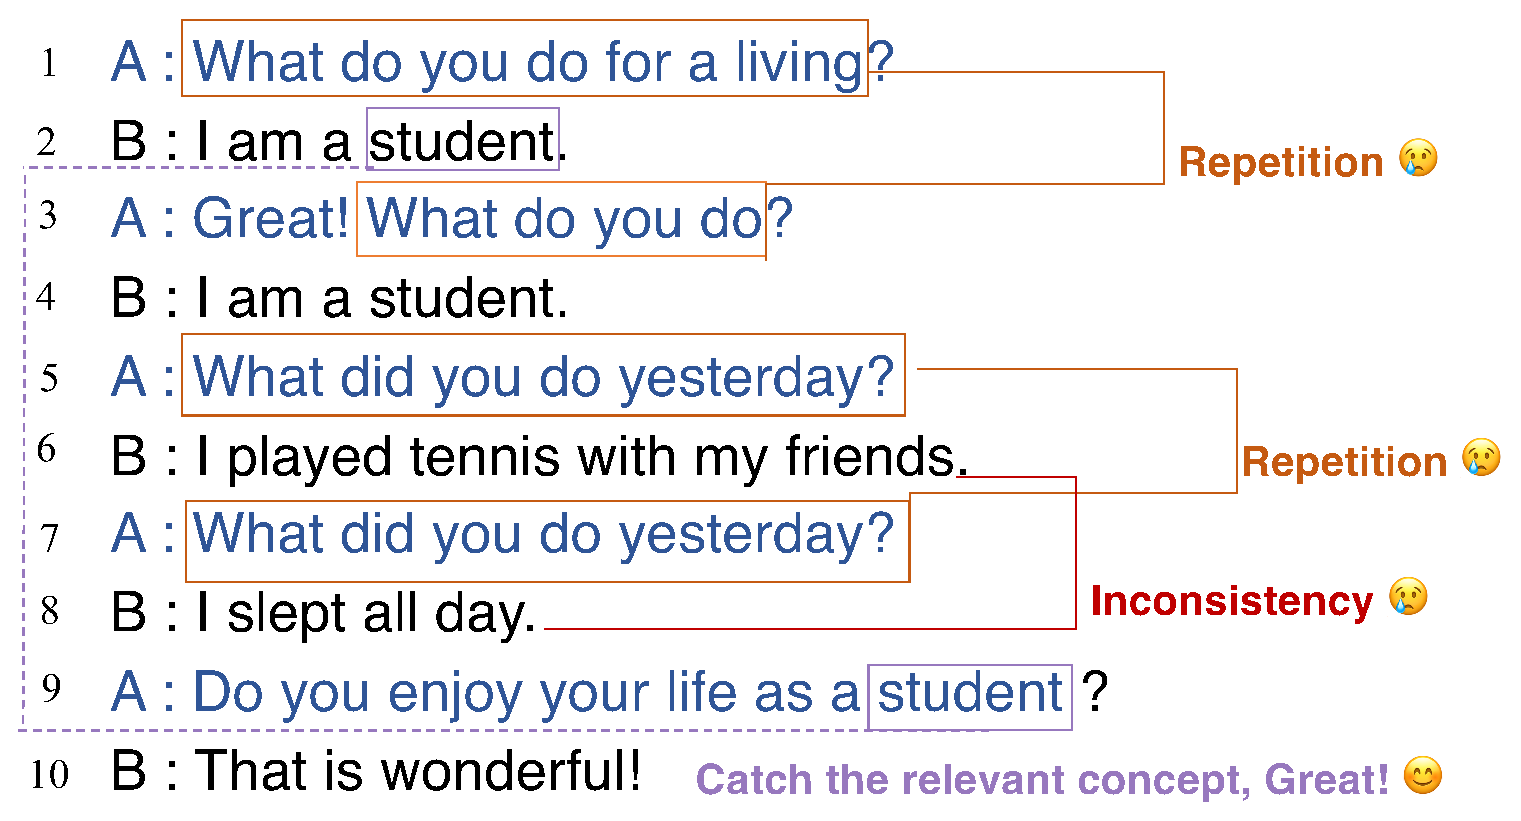
\includegraphics[width=0.95\columnwidth]{example2.eps}
        \caption{A chat snippet between two bots.}
        \label{fig:example}
\end{figure}

Fluency, Knowledge, Proactivity and Specificity are scored for each turn separately
and aggregated at the end of the conversation.
Detection for diversity, consistency and relevance are more involved and are explained
using \figref{fig:example}. 

As for diversity, at each turn $t$, we first check if there exists any repetitive question.  
We can easily find turn 3 and turn 7 repeated turn 1 and turn 5 
respectively. They will then be penalized one point for repetition. 
Repetition is not penalized if the previous turn is already 
marked as a repetitive question. For example, in \figref{fig:example}, 
although turn 4 is considered a repetition of turn 2,  
we are not going to penalize it as turn 3 is a repetitive question. 

The detection of inconsistency is always triggered after the detection of repeated questions. 
If the answers to the same questions are different, we will penalize the current turn, 
such as turn 8 in \figref{fig:example}.

We decide a repetition or an inconsistency by calculating the similarity of the two turns. 
We use a similarity function to complete the calculations, which we will 
discuss in \secref{sec:experiment}. The actual diversity and consistency scores
are the negation from the amount of repetition and inconsistency.

Relevance is assessed as a bonus to reward
a bot if it is able to memorize the important relevant concepts that have shown up 
before in the conversation. We sort the concepts that have shown up in 
chat history by their IDF scores. For example, in turn 9, $A$ 
mentions the concept word ``student'' presented by $B$ in turn 2. With this
turn, $A$ will win a bonus point.


The algorithms and notations for computing diviersty, consistency and relevance are included
in \tabref{tab:functions}, \algoref{algo:rep}, \algoref{algo:inconsist}, and \algoref{algo:bonus}. 

\begin{table}[th]
\centering
\small
\begin{tabular}{c|l}
%\hline
\toprule
\textbf{Notation} & \textbf{Description} \\ \midrule
$t$ & Current turn \\
$H(t)$  &  a list of history turns prior to $t$ \\
$Sim(x,y)$ & similarity between two turns $x$ and $y$ \\
$\sigma_r$ & Threshold for detecting repetition \\
$\sigma_c$ & Threshold for detecting consistency \\
$r$ & Weight for repetition \\
$c$ & Weight for inconsistency \\
$b$ & Weight for bonus \\
$d$ & Min distance between consecutive mentions \\
IDF list & List of lemma in chatlog sorted by IDF\\
$p$ & Percentage of important lemmas in IDF list\\
$R(t)$ &  Repetition penalty for turn $t$ \\
$C(t)$ &  Inconsistency penalty for turn $t$ \\ 
$B(t)$ &  Memory bonus for turn $t$ \\
$Rep(t)$ & A list of repeated turns for turn $t$ \\  
\bottomrule
\end{tabular}
\caption{
Functions and variables in algorithms.}
\label{tab:functions}
\end{table}

\begin{algorithm}[th]
\small
\caption{Scoring for Diversity}
\label{algo:rep}
\hspace*{0.02in} {\bf Input:}
 $t$, $H$, $Sim$, $\sigma_{r}$
; \hspace*{0.02in} {\bf Output: } 
 $R$;
\begin{algorithmic}[1]
\State //Starting to detect repetition
\For {$u$ in $H(t)$}
	\If {$Sim(t,u) \geq \sigma_{r}$}
		\State Add $u$ to $Rep(t)$
	\EndIf
\EndFor
    \If{$len(Rep(t))\geq 0$}
        \If{$t$ is a question and We can find a question in $Rep(t)$}
        \State $ R(t) \leftarrow  R(t) + 1$ 
        \Else
        \If {the previous turn of $t$ is not a repetitive question}
        \State $R(t)) \leftarrow R(t) + 1$ 
        \EndIf
        \EndIf
    \EndIf
\end{algorithmic}
\end{algorithm}


\begin{algorithm}[th]
\small
\caption{Scoring for Consistency}
\label{algo:inconsist}
\hspace*{0.02in} {\bf Input:}
$t$, $H$, $Sim$, $\sigma_{c}$
; \hspace*{0.02in} {\bf Output:  } 
 $C$;
\begin{algorithmic}[1]
\State // Inconsistency detection
 \If {previous turn of $p$ is a repetitive question} 
   \If{ the response $res$ to the question repeated by turn $p$ contradicts turn $i$ with $Sim(t, res) \leq \sigma_{c}$ }
    \State $C(t) \leftarrow C(t) + 1$
   \EndIf
  \EndIf
\end{algorithmic}
\end{algorithm}

\begin{algorithm}[th]
\small
\caption{Scoring for Relevance}
\label{algo:bonus}
\hspace*{0.02in} {\bf Input:}
$t$, $p$, $d$
; \hspace*{0.02in} {\bf Output:  } 
$B$;
\begin{algorithmic}[1]
\State // Assessing the ability of catching relevant concepts\\
$B(t) \leftarrow 0$
\For {all tokens $tk$ in current turn $t$}
 \If {$t$ - previous occurrence turn of $tk > d$ and $tk$ in the top $p\%$ of the IDF list of all tokens in the dialogue} 
   \State $B(t) \leftarrow 1$
  \EndIf
 \EndFor
\end{algorithmic}
\end{algorithm}

At the end of each game, each bot gets seven scores, one for each dimension.  
After pairwise comparison on individual dimension, a bot gains one point for win and zero point for a tie or lose.
The final score of each bot is determined by the sum of their individual scores.
%\KZ{Are these scores positive or negative? Comparable between bots?}

\subsubsection*{Match-level Scoring}
%\KZ{Use an equation to compute the final scores?}
One match which consists of two games, each started with a different bot, 
decides winning or losing between two bots.
For match-level scoring, we mimic the scoring rules of soccer tournament. 
For each match, $W$ points for the winner,  
$T$ points for a tie and 
$L$ points for the loser.
The value of $W$, $T$ and $L$ will be discussed in \secref{sec:ablation}. 

%\KZ{At the match level, we need to consider different starting context for the bots? I think we should present a few options for the reader and say that we are limited to these.}

\subsubsection*{Tournament-level Scoring}
%\KZ{Use an equation to compute the final scores?}
We count the points by simply summing up their scores gained in every match. Currently, several bots with the same final rank are tolerated. For future study, it's possible to mimic more detailed rules presented in sports match such as determine their ranking based on their win-loss relationship in the match between them.  
If they are still tied, we could propose an “overtime” for these two bots, one human judge may observe their performance and then make the decision of the game.

\section{Experiment}
In this section, we experiment on different NLG tasks. We first present the experimental setup on different tasks. Then, we show the quantitative and qualitative results together with comprehensive analysis and ablation studies.

\subsection{Implementation Details}
We evaluate the newly proposed ICL strategy on five commonly-researched natural language generation tasks: reading comprehension, dialogue summarization, style transfer, question generation and news summarization. Details on the task description, the strong baseline, corresponding  dataset, evaluation metrics and key hyper-parameters for each task are presented as follows.

\begin{table*}[th]
	\scriptsize
	\centering
	\begin{tabular}{lp{1.1cm}rrrcccc}
		\hline
		Task & Dataset & \#Train & \#Val & \#Test & Input & Output & Avg & Std\\
		\hline
		Reading Comprehension & DREAM & 6,116 & 2,040 & 2,041 & ``Q:''+ question + dialogue & answer & 5.59 & 2.61\\
		Dialogue Summarization & SAMSum & 14,732 & 818 & 819 & dialogue & summary  & 24.99 & 13.06\\
		Style Transfer & Shakespeare & 36,790 & 2,436 & 2,924 & original/modern  & modern/original  & 11.63 & 8.19 \\
		Question Generation & SQuAD1.1 & 75,722 & 10,570 & 11,877 & passage + [SEP] + answer & question & 13.09 & 4.27 \\
		News Summarization & CNNDM & 287,227& 13,368& 11,490 & document & summary & 70.97 & 29.59\\ 
		\hline
	\end{tabular}
	\caption{A summary of tasks and datasets. \#Train, \#Val and \#Test refers to the number of samples in the corresponding dataset. Avg and Std are the statistics for the number of output tokens. ``+'' refers to the concatenation operation.}
	\label{tab:taskdata}
\end{table*}

\textbf{Reading comprehension} is the task that answering questions about a piece of text. We use the DREAM dataset~\cite{sun2019dream} where questions are about corresponding dialogues and the answer is a complete sentence in natural language. We neglect the negative choices in the original dataset and formulate it as a NLG task. We adopt the pre-trained language model BART~\cite{lewis2020bart} as the baseline, where the input is a concatenation of a question and the corresponding dialogue made up of speakers and utterances. 
We experiment with  transformers\footnote{\url{https://github.com/huggingface/transformers}} based on the publically available ``facebook/bart-large'' checkpoint \footnote{\url{https://huggingface.co/facebook/bart-large}}.
%The preceding BART model is also adopted as the baseline, whereas the input is a concatenation of question and a dialogue.
The generated answers are evaluated by BLEU scores\footnote{The BLEU-1/2/3/4 scores are computed according the Google's implementation(\url{https://github.com/tensorflow/nmt/blob/master/nmt/scripts/bleu.py}).}~\cite{papineni2002bleu} widely used for QA systems, together with Meteor and Rouge-L F1 as mentioned above. The parameters are also the same as dialogue summarization, except that the early-stop is activated if there is no improvement on the perplexity of the validation set. 


\textbf{Dialogue summarization} is to generate a concise summary covering the salient information in the input dialogue. The preceding model BART has shown to be a strong baseline for this task, where only the dialogue is concatenated into a single sequence as the input. We experiment with  %transformers\footnote{\url{https://github.com/huggingface/transformers}} based on the publically available ``facebook/bart-large'' checkpoint \footnote{\url{https://huggingface.co/facebook/bart-large}} and 
SAMSum dataset\footnote{\url{https://arxiv.org/src/1911.12237v2/anc/corpus.7z}}~\cite{gliwa2019samsum} for daily-chat dialogues. 
The generated summaries are evaluated by comparing with the reference through evaluation metrics, including Rouge-1/2/L F1 scores\footnote{\url{https://github.com/pltrdy/files2rouge}}~\cite{lin2004rouge}, Meteor~\cite{banerjee2005meteor} and BertScore F1\footnote{Both Meteor and BertScore are calculated by SummEval(\url{https://github.com/Yale-LILY/SummEval}), and the latter one is based on the default bert-base-uncased model.}. We evaluate the model on the validation set after each training epoch and the early-stop patience will be added 1 if there is no improvement according to the Rouge-2 F1 score. The training process terminates when the early-stop patience equals or is larger than 3.  During the inference, the minimum and maximum output length is set to 5 and 100 respectively, with no\_repeat\_ngram\_size=3, length\_penalty=1.0 and num\_beams=4.


% The answer is either a span of words in the original text or a complete sentence in natural language.
\textbf{Style transfer} preserves the semantic meaning of a given sentence while modifies it's style, such as positive to negative, formal to informal, etc.
We adopt the Shakespeare author imitation dataset~\cite{xu2012paraphrasing}, containing William Shakespeare's original plays and corresponding modernized versions. Krishna el al.~\shortcite{krishna2020reformulating} proposed to do unsupervised style transfer by training paraphrase models based on the GPT-2 language model~\cite{radford2019language}. We re-implemented their approach STRAT\footnote{\url{https://github.com/martiansideofthemoon/style-transfer-paraphrase}} and evaluated with the provided script. Evaluation metrics includes 
transfer accuracy(ACC), semantic similarity(SIM), Fluency(FL) and two aggregation metrics, i.e., geometric averaging(GM) and their newly introduced $J(\cdot)$ metric. The hyper-parameter $hp$ equaling 0.0, 0.6 or 0.9  in Table~\ref{tab:end2endst} is the sampling parameter for trades off between ACC and SIM in their approach. 
In the training stage, we evaluate the model after updating every 500 steps. The perplexity on the validation set is used to activate the early-stop which equals 3. The inference is done as default.
 
\textbf{Question generation}~\cite{zhou2017neural} aims at generating a question given an input document and its corresponding answer span. SQuAD 1.1~\cite{rajpurkar2016squad} is generally used for evaluation. We adopt the data split as in \cite{du2017learning} and fine-tune the pre-trained UniLM~\cite{dong2019unified} as the strong baseline according to their official implementation\footnote{\url{https://github.com/microsoft/unilm/tree/master/unilm-v1}}. Generated questions are evaluated by metrics including BLEU-1/2/3/4, Meteor and Rouge-L with the provided scripts. The model is evaluated every 1000 steps and the early-stop equaling 3 is associated with the perplexity on the validation set. Other parameters are unchanged following the official guideline.

\textbf{News summarization} differs from dialogue summarization where the input is a document instead of a dialogue. We adopt the same strong baseline BART and evaluation metrics as dialogue summarization. Experiments are done with CNNDM dataset~\cite{HermannKGEKSB15} consisting of news articles and multi-sentence summaries\footnote{\url{https://github.com/pytorch/fairseq/blob/main/examples/bart/README.summarization.md}}. The model is evaluated every 2000 steps and the early-stop equaling 3 is associated with the Rouge-2 on the validation set. During the inference, the minimum and maximum output length is set to 45 and 140 respectively, with no\_repeat\_ngram\_size=3, length\_penalty=2.0 and num\_beams=4.
%\footnote{Inference parameters are borrowed from \url{https://github.com/pytorch/fairseq/blob/main/examples/bart/summarize.py}}

The summary of each task is listed in Table~\ref{tab:taskdata}. For fair comparisons, we re-implemented baselines following the above instructions on our machine. On top of the above baselines, we further arm them with the ICL strategy according to the Algorithm~\ref{alg:picl}. The settings of newly introduce Start and Stride are specified and discussed in following sub-sections. All of our experiments are done on a single RTX 3090 or a single RTX 2080Ti with 24G and 11G GPU memory respectively.
%and the result are averaged over three runs.


 
\subsection{Automatic Evaluations on Different Tasks}
\label{sec:taskperformances}

We compare our approach with the vanilla models mentioned above and the approach from~\citet{liang-etal-2021-token-wise} as baselines.
The performances on different NLG tasks are shown in Table~\ref{tab:end2end}. 
These tasks not only focus on solving different problems, but also has various amount of training data as well
as reference output lengths as shown
Table~\ref{tab:taskdata}.
Besides, the basic model are also different, including BART, GPT-2 and UniLM. 
Our new training strategy achieves significantly improvements among different tasks on most evaluation metrics, which shows that our method not only works well, but also has strong generalization abilities.

We explain the some specific results as follows:

(1) Our training strategy boosts the performances of the original STRAT with different $hp$ in the style transfer task. GM and J are two comprehensive evaluation metrics, with our approach topping the ranks with significant improvements.

(2) TCL generally performs poorly on tasks
with more training data. For example, it failed on question generation without any improvements over the vanilla model under the same parameter setting, while ICL still 
logs gains. This is mainly due to two reasons.
First, because the nature of TCL is data augmentation which is more effective in low-resource settings,
when training data is abundant, it becomes less useful. 
Second, the way they calculate the loss as sub-sequence generation better suites paraphrasing tasks, such as machine translation tested in their paper, as the order of 
the corresponding tokens between input and output 
are almost the same. Learning such forward mapping can 
be regarded as a kind of ``easy-to-hard'' 
in these limited scenarios.
However, this doesn't hold true for other tasks, 
such as summarization and question generation. 
Therefore, we didn't further test it on CNNDM since
CNNDM has the large amount of training data among
the five.

(3) For news summarization, Rouge-1 scores (precision, recall) for the baseline and our method on CNNDM are (38.16, 52.72) and (40.84, 49.23) correspondingly. Our method made substantial improvements on the precision with a compromise on the recall. 
The meteor score based on the unigram precision and recall emphasizes more on the recall than the Rouge-1 F1. As a result, it drops while Rouge-1 F1 increases. Overall, our method still outperforms BART on this task, especially on F1 scores of Rouge-2 and Rouge-L.




\begin{table}[th]
	\small
	\centering
	\begin{subtable}{\linewidth}
		\scriptsize
		\centering
		\begin{tabular}{lcccccc}
			\hline
			{Method} & {B1} & {B2} & {B3} & {B4} & {Met} & {RL}\\
			\hline
			w/o CL &  32.03 & 16.01 & 8.77 & \textbf{4.80} & 19.84 & 38.89\\
			TCL & 32.53 & 16.25 & 8.52 &4.67 &19.88 & 39.65 \\
			ICL &  \underline{\textbf{33.99}} & \underline{\textbf{17.43}} & \underline{\textbf{9.18 }}& 4.64 & \textbf{20.60} & \textbf{40.78}\\

			\hline
		\end{tabular}
		\caption{Reading Comprehension}
		\label{tab:end2endrc}
	\end{subtable}
	\\[5pt]
	\begin{subtable}{\linewidth}
		\scriptsize
		\centering
		\begin{tabular}{lccccc}
			\hline
			{Method} & {R1} & {R2} & {RL} & {Met} & {BertS} \\
			\hline
			%BART & 52.60&27.00 &42.10 &- & - \\
			w/o CL & 51.88 & 27.30 & 42.77 & 24.75 & 71.38 \\
			TCL  & 52.33 & 27.80 & \textbf{43.91} & 24.59 & 71.77 \\
			ICL & \underline{\textbf{53.07}} & \underline{\textbf{28.23}} & {43.83} & \underline{\textbf{26.12}}& \underline{\textbf{72.17}} \\
			
			\hline
		\end{tabular}
		\caption{Dialogue Summarization}
		\label{tab:end2endds}
	\end{subtable}
	\\[5pt]
	\begin{subtable}{\linewidth}
		\scriptsize
		\centering
		\begin{tabular}{lcccccc}
			
			\hline
			{Method}&$hp$ &  {ACC} & {SIM} & {FL} & {GM} & {J}\\
			\hline
			%\multirow{3}{*}{STRAT}& 0.0 & 71.70 & \textbf{56.40} & 85.20 & 70.10 & 34.70 \\
			%& 0.6 & 75.70 & 53.70 & 82.70 & 69.50 & 33.50 \\
			%& 0.9 & 79.80 & 47.60 & 71.70 & 64.80 & 27.50 \\
			%\hline
			\multirow{3}{*}{w/o CL}& 0.0 & 70.49 & 55.70 & 85.98 & 69.63& 33.72 \\
			& 0.6 &75.31 & 53.46 & 82.56 & 69.27& 33.30\\
			& 0.9 & 78.76 & 47.38 & 74.42 &65.24 & 27.88\\
						\hline
			\multirow{3}{*}{TCL } & 0.0 & 70.31 & \textbf{55.95} &\textbf{87.24} &  70.01& 34.71 \\
			& 0.6 & 74.79 & 53.14 & 82.56 & 68.97 & 33.21 \\
			& 0.9 & 79.41 & 46.88 & 71.92 &64.45 & 26.92 \\
			\hline
			\multirow{3}{*}{ICL}& 0.0 & \underline{73.72} & 55.91 & 86.30 & \underline{\textbf{70.60}} &\underline{\textbf{35.81}}\\
			& 0.6 & 77.26 & \underline{53.80} & \underline{83.87} & \underline{70.38} & 34.64\\
			& 0.9 & \textbf{79.65} & 48.16 & 76.06 & 66.32 & 29.03\\

			\hline
		\end{tabular}
		\caption{Style Transfer.}
		\label{tab:end2endst}
	\end{subtable}
	\\[5pt]
	\begin{subtable}{\linewidth}
		\scriptsize
		\centering
		\begin{tabular}{lcccccc}
			\hline
			{Method} & {B1} & {B2} & {B3} & {B4} & {Met} & {RL}\\
			\hline
			w/o CL & \textbf{50.38} & 35.67 & 27.24 & 21.36 & 24.40 & 50.67 \\
			TCL &\textbf{50.38} & 35.67 & 27.24 & 21.36 & 24.40 & 50.67\\
			ICL &  50.18 & \textbf{35.72} & \textbf{27.36} & \textbf{21.54} & \textbf{24.57} & \underline{\textbf{51.09}} \\
			\hline
		\end{tabular}
		\caption{Question Generation}
		\label{tab:end2endqg}
	\end{subtable}
		\\[5pt]
	\begin{subtable}{\linewidth}
		\scriptsize
		\centering
		\begin{tabular}{lccccc}
			\hline
			{Method} & {R1} & {R2} & {RL} & {Met} & {BertS}\\
			\hline
			%BART &  \\
			w/o CL &  43.07 & 20.01 & 35.94 & \textbf{21.44} & 63.72 \\
			TCL & - & -&- &- &- \\
			ICL & \textbf{43.39} & \underline{\textbf{20.55}} & \underline{\textbf{36.63}} & 19.68 & \textbf{64.05}\\
			\hline
		\end{tabular}
		\caption{News Summarization}
		\label{tab:end2endns}
	\end{subtable}
	\caption{Performances on different NLG tasks. ICL represents the models trained with our ICL algorithm. TCL refers to the previous work from~\cite{liang-etal-2021-token-wise}. Scores underlined are statistically significantly better than both re-implemented baselines with $p<0.05$ according to t-test. }	
	\label{tab:end2end}
\end{table}


\subsection{Human Evaluations}

To further prove the improvement of ICL, we hired three proficient English speakers for human evaluation. 20 samples from the test set of each task are randomly selected, ignoring the ones with totally same generations among three models, including the vanilla model, TCL and ICL. The original input, reference output and three generations are shown to annotators together, while the order of three generations are unknown and different among samples. 3-point Likert Scale is adopted for scoring for each generation~\cite{gliwa2019samsum}, where [1, 3, 5] represent 
excellent, moderate and disappointing results 
respectively. The average scores and agreements 
among the annotators are shown in 
Table~\ref{tab:humaneval}.

The Fleiss Kappa on the first four tasks indicates the fair to moderate agreements. It shows the promising improvement of ICL over the vanilla model and TCL especially on DREAM, SAMSum, and SQuAD1.1, which is consistent with the conclusion based on automatic metrics.
Although the agreement on style transfer is fair, 
our annotators without Shakespeare background 
tend to give low scores to all outputs.
Therefore, the absolute improvement is 
only $0.04$ compared to both baselines.
%This mainly due to the indistinguishable styles between
%Shakespeare’s plays with are quite different from modern languages. 
Besides, the poor agreement on CNNDM reflects the 
diverse concerns of summarization from different 
annotators. Without more specific instructions, they 
tends to focus more on the content coverage instead 
of checking the detailed facts. This is also 
consistent with the higher Meteor scores of the 
vanilla model over ICL.

\begin{table}[th]
	\scriptsize
	\centering
	\begin{tabular}{l|ccc|c}
		\hline
		{Datasets} & {w/o CL} & {TCL} & {ICL} & {Agreement}  \\
		\hline
		DREAM  &3.07 & 2.50&3.20 &0.48 \\
		SAMSum &2.97 &3.57 &3.97 &0.40 \\
		Shakespeare &2.23 &2.23 & 2.27&0.32 \\
		SQuAD1.1 &3.43 & 3.43 &3.77 &0.35 \\
		CNNDM & 3.45 &- &3.40 &0.11 \\
	%	\hline
	%	overall & & & &\\
		\hline
	\end{tabular}
	\caption{Human evaluations. The agreement is calculated by Fleiss Kappa.}
	\label{tab:humaneval}
\end{table}




%Following Liu et al.\shortcite{liu2021competence}'s work, we asked annotators to comparing the performance between our generated results and baselines by choosing from ``Better, Tie, Worse''. 
%The counts for each choice are shown in Table~\cite{}, where the Fleiss Kappa among annotators is ??.

%Analysis





%\subsection{Analysis on Variable Generation Lengths}

%Teacher forcing, which predicts each token given the reference summary tokens during training and given the previous generated tokens during inference, leads to the exposure bias problem for NLG tasks.
%Since ICL starts the training process by predicting the last few tokens of outputs and gradually calculates the loss based on more tokens when the model is stronger, we hypothesis that it can alleviate the exposure bias for training Seq2Seq models to some extent.
%As stated in~\cite{pang2020text}, the output quality tends to degrade as the output length increase with the exposure bias.
%So, we divided the test set of each task according to the length of the generated output into 4 buckets and randomly picked 20 samples in each buckets for both the corresponding baselines and our approach. Each generation is annotated by 5 point Likert Scale, where 1 is the worst and 5 is the best. 

%The trends of performances on variable generation lengths are in Figure~\ref{}.


\section{Related Work}
This section surveys previous works on question generation and tree encoding
respectively.

Text question generation has attracted the attention 
after the work of ~\citeauthor{du2017learning}~\shortcite{du2017learning}, who uses deep seq2seq model 
to generate questions from a raw text paragraph. 
Before that, text question generation relied heavily on hand-craft 
question patterns~\cite{HeilmanS10,LabutovBV15,MostowC09} which is time and 
labor consuming. 

However, this pure seq2seq model is not focused and 
has no control over part in the paragraph to generate question. 
~\citeauthor{zhou2017neural}~\shortcite{zhou2017neural} proposed to encode 
key phrase information using binary indicators to generate 
key-aware questions and they assumes the answer to be key phrase. 
Considering key phrase (answer) is unavailable in reality, 
~\citeauthor{SubramanianWYT17}~\shortcite{SubramanianWYT17} applied 
a two-stage approach. First, key phrases are extracted by 
pointer network~\cite{ptrnet}. Second, 
key phrases are encoded in the same way as 
Zhou et al. With the intuition that questions could be asked in many ways, 
~\citeauthor{Yao2018vae}~\shortcite{Yao2018vae} used conditional-VAE to 
increase the diversity of questions. More recently, models with 
auxiliary feature information~\cite{HarrisonW18} helped improve 
the question quality. Structure question generation aims at 
converting structured data such as triples in knowledge graph to questions. 
~\citeauthor{SerbanGGACCB16}~\shortcite{SerbanGGACCB16} proposed a model to generate factoid questions from knowledge base triples.  None of the above work
considered using parse tree structures to aid question generation process,
which is the focus of this paper.

Sequential RNN model takes sentence as a sequence of words, 
ignoring the syntactic information. In order to utilize
such syntactic information with sequential information, 
~\citeauthor{tai2015improved}~\shortcite{tai2015improved} proposed Tree-LSTM to 
encode the binary parse tree recursively in a bottom-up fashion to 
classify sentiment. In text generation task, 
\citeauthor{eriguchi2016tree}~\shortcite{eriguchi2016tree} 
proposed a tree-to-sequence model with attention mechanism to do 
machine translation and 
~\citeauthor{liang2018automatic}~\shortcite{liang2018automatic} proposed a 
tree-to-sequence model which could handle arbitrary trees, 
to do code comment generation. Our work is inspired by these previous
attempts and we are first to adapt structure encoded neural models to
textual question generations.
\section{Conclusion}
\label{sec:conclude}
In this work,
we propose a new data creation method to generate
 a semi-structured synthetic training data for 
opinion summarization,
which is known for lacking training data.
\cut{We showed that by extracting an aspect-opinion pairs and 
implicit sentences from multiple reviews
first and then synthesizing them into semi-structured data, we achieve
better performance on opinion summarization.}
%\KZ{It is critical to show in your experiments that the proposed
%synthetic data is better than other possible alternatives.}, 
We also designed an aspect-guided model with opinion-aspect pair encoder and implicit sentence encoder.
The results showed that
the proposed model can make full use of semi-structured data
and generate high-quality summaries.




\section*{Acknowledgment}
Kenny Q. Zhu is the contact author and was supported by NSFC grants 
91646205 and 61373031. Thanks to the anonymous reviewers for their valuable 
feedback.

%\bibliographystyle{acl}
\bibliography{emnlp2018}
\bibliographystyle{acl_natbib_nourl}

\end{document}
